\chapter{Verwendete Technologien}\label{cha:used-technologies}

\section{Over The Air Update (OTA)}\label{sec:ota}

\subsection*{Problemstellung}\label{sec:problem}
Mikrocontroller befinden sich, wenn sie sich in einem laufendem System befinden meist an ungünstigen Orten, an die man nur mit hohem Aufwand gelangt.
Bis jetzt musste man den Computer physisch mit einem Kabel mit dem Mikrocontroller verbinden um neue Firmware auf den Kontroller zu spielen.
OTA ermöglicht es den Mikrocontroller über das Netzwerk mit neuer Firmware zu versorgen, dabei muss der selektierte Microcomputer lediglich mit einem Wlan-Router verbunden sein und ein physisches Kabel wird überflüssig.

\subsection*{Wie OTA funktioniert}
Bei dem OTA-Vorgang wird zuerst die Config-Datei, des jeweiligen Mikrocontrollers, ausgelesen. In dierser Config-Datei steht auch welches Firmware sich OTA herunterladen soll. Nun überprüft der Mikrocontroller ob die Firmware-Version des Servers neuer ist als die, die der Controller bereits besitzt, ist dies der Fall wird die neue Version heruntergeladen und der Mikrocontroller wird mit der aktuellen Version neu gestartet.

\subsection{Partitions Tabelle}
Die Partitionstabelle ist bei OTA mitunter eines der wichtigsten Themen. Würde man diese Tabelle nicht richtig konfigurieren würde das Programm nicht einmal starten. Dazu kommt noch eine erschwerte Fehlersuche, da Errormeldungen bei der Arbeit mit Mikrocontrollern zu wünschen lassen.
Die Standard-Partitionstabelle ist je nach Hersteller anders. Um OTA zu ermöglichen ist es notwendig im Partitionstabelle mindestens eine, ausreichend große, OTA-Partition zu vergeben. Dabei ist es wichtig, dass diese Partition ausreichend Speicher für die gewünschte Firmware hat, da sonst der ganze Vorgang abgebrochen wird.

\subsubsection{Übersicht}
Der Flash eines einzelnen ESP32 kann mehrere Apps sowie viele verschiedene Arten von Daten (Kalibrierungsdaten, Dateisysteme, Parameterspeicherung usw.) enthalten. Aus diesem Grund wird eine Partitionstabelle im Flash auf (Standardoffset) 0x8000 geflasht.

Die Länge der Partitionstabelle beträgt 0xC00 Byte (maximal 95 Partitionstabelleneinträge). Nach den Tabellendaten wird eine MD5-Prüfsumme angehängt, mit der die Integrität der Partitionstabelle überprüft wird. Wenn die Partitionstabelle aufgrund eines sicheren Starts signiert ist, wird die Signatur nach der Partitionstabelle angehängt.

Jeder Eintrag in der Partitionstabelle hat einen Namen (Bezeichnung), einen Typ (app, data, ota oder etwas anderes), einen SubType und den Offset im Flash, in dem die Partition geladen wird.

\subsubsection{Custom Partition Tables}
Bei komplexeren Anwendungen reichen die default Partitionstabellen nicht mehr aus und es muss eine angepasste Tabelle erstellt werden, welche aber auch genau auf die Bedürfnisse von gewissen Firmwares zugeschnitten werden kann.

Wenn die Option der Benutzerdefinierte Partitionstabelle ausgewählt wird. Muss manuel eine CSV-Datei erstellt werden, in der dann eine beliebige Anzahl von Partitionen mit folgenden Punkten eingetragen werden können:

\begin{itemize}
    \item Name
    \item SubType
    \item Offset
    \item Size
    \item Flags
\end{itemize}

\begin{figure}[H]
    \begin{center}
        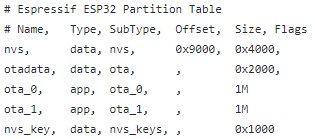
\includegraphics[scale=1]{images/partition_table.png}
        \caption{Beispiel Partitionstabelle (Quelle: eigene Darstellung)}
    \end{center}    
\end{figure}

\subsubsection{Name Feld}
Das Namensfeld kann beliebig gewählt werden. Es ist für den Mikrocontroller nicht von Bedeutung. Namen die länger als 16 Zeichen sind werden jedoch abgeschnitten.

\subsubsection{Type Feld}
Das Partitionstypfeld kann als App (0) oder Daten (1) angegeben werden. Oder es kann eine Zahl 0-254 sein (oder als Hex 0x00-0xFE). Die Typen 0x00-0x3F sind für esp-idf-Kernfunktionen reserviert.

Wenn eine Anwendung Daten speichern muss, muss einen benutzerdefinierten Partitionstyp im Bereich 0x40-0xFE hinzugefügt werden.

Der Bootloader ignoriert alle anderen Partitionstypen als App (0) und Daten (1).

\subsubsection{SubType}
Das 8-Bit-SubType-Feld ist spezifisch für einen bestimmten Partitionstyp. Esp-idf gibt derzeit nur die Bedeutung des Subtypfelds für die Partitionstypen "App" und "Daten" an (Stand 09.03.2020).


Wenn der Typ "App" ist, kann das Subtypfeld als Factory (0), ota\_0 (0x10) ... ota\_15 (0x1F) oder test (0x20) angegeben werden.
factory (0) ist die Standard-App-Partition. Der Bootloader führt die Factory-App aus, es sei denn, er sieht eine Partition vom Typ data / ota. In diesem Fall liest er diese Partition, um zu bestimmen, welches OTA-Image gestartet werden soll.
OTA aktualisiert niemals die Factory-Partition.
Wenn Sie die Flash-Nutzung in einem OTA-Projekt beibehalten möchten, können Sie die Factory-Partition entfernen und stattdessen ota\_0 verwenden.
ota\_0 (0x10)\dots ota\_15 (0x1F) sind die OTA-App-Slots. Verwenden Sie dann die OTA-Datenpartition, um zu konfigurieren, welchen App-Slot der Bootloader starten soll. Wenn Sie OTA verwenden, sollte eine Anwendung mindestens zwei OTA-Applikationslots haben (ota\_0 und ota\_1).
test (0x20) ist ein reservierter Subtyp für werkseitige Testverfahren. Es wird als Fallback-Boot-Partition verwendet, wenn keine andere gültige App-Partition gefunden wird. Es ist auch möglich, den Bootloader so zu konfigurieren, dass er bei jedem Start einen GPIO-Eingang liest, und diese Partition zu starten, wenn der GPIO "low" gehalten wird.
Wenn der Typ "data" ist, kann das Subtypfeld als ota (0), phy (1), nvs (2) oder nvs\_keys (4) angegeben werden.
ota (0) ist die OTA-Datenpartition, in der Informationen zur aktuell ausgewählten OTA-Anwendung gespeichert werden. Diese Partition sollte mindestens 0x2000 Bytes groß sein.
phy (1) dient zum Speichern von PHY-Initialisierungsdaten.
In der Standardkonfiguration wird die Phy-Partition nicht verwendet und die PHY-Initialisierungsdaten werden in der App selbst kompiliert. Daher wird diese Partition aus Platzgründen meist aus der Partitionstabelle entfernt.
nvs (2) steht für die NVS-API (Non-Volatile Storage).
NVS wird zum Speichern von PHY-Kalibrierungsdaten pro Gerät verwendet (anders als Initialisierungsdaten).
NVS wird unter anderem zum Speichern von WiFi-Daten verwendet, wenn die Initialisierungsfunktion esp\_wifi\_set\_storage (WIFI\_STORAGE\_FLASH) verwendet wird.
Die NVS-API kann auch für andere Anwendungsdaten verwendet werden.
Es wird dringend empfohlen, eine NVS-Partition von mindestens 0x3000 Byte in Ihr Projekt aufzunehmen, da sonst einige unerwartete Fehler auftreten können.
Wenn Sie die NVS-API zum Speichern vieler Daten verwenden, erhöhen Sie die NVS-Partitionsgröße von den standardmäßig 0x6000 konfigurierten Bytes.
nvs\_keys (4) ist für die NVS-Key-Partition.
Es wird zum Speichern von NVS-encryption-keys verwendet, wenn das NVS Encryption feature aktiviert ist.
Die Größe dieser Partition sollte 4096 Byte betragen (minimale Partitionsgröße).

\subsection{Offset}
Partitionen mit leeren Offsets beginnen nach der vorherigen Partition oder nach der Partitionstabelle bei der ersten Partition.

App-Partitionen müssen an Offsets sein, die auf 0x10000 (64 KB) ausgerichtet sind. Wenn das Offset-Feld leer gelassen wird, richtet gen\_esp32part.py die Partition automatisch aus. Wenn ein nicht ausgerichtetes Offset für eine App-Partition angegeben wird, wird ein Fehler generiert.

Größen und Offsets können als Dezimalzahlen, Hexadezimalzahlen mit dem Präfix 0x oder Größenmultiplikatoren K oder M (1024 und 1024 * 1024 Byte) angegeben werden.

Wenn Sie möchten, dass die Partitionen in der Partitionstabelle mit einem Startoffset (CONFIG\_PARTITION\_TABLE\_OFFSET) der Tabelle selbst funktionieren, lassen Sie das Feld Offset (in der CSV-Datei) für alle Partitionen leer.

\subsubsection{Flags}
Derzeit wird nur ein Flag unterstützt: encrypted. Wenn dieses Feld auf encrypted eingestellt ist, wird diese Partition verschlüsselt, wenn die Flash-Verschlüsselung aktiviert ist.

Partitionen vom App-Typ werden immer verschlüsselt unabhängig ob die Flag gesetzt ist oder nicht.
\cite{espressif_partition_tables}
\subsection*{Implementation}
Die ausgewählte Struktur für die Diplomarbeit kann man im folgenden Bild sehr gut sehen.

\begin{figure}[H]
    \begin{center}
        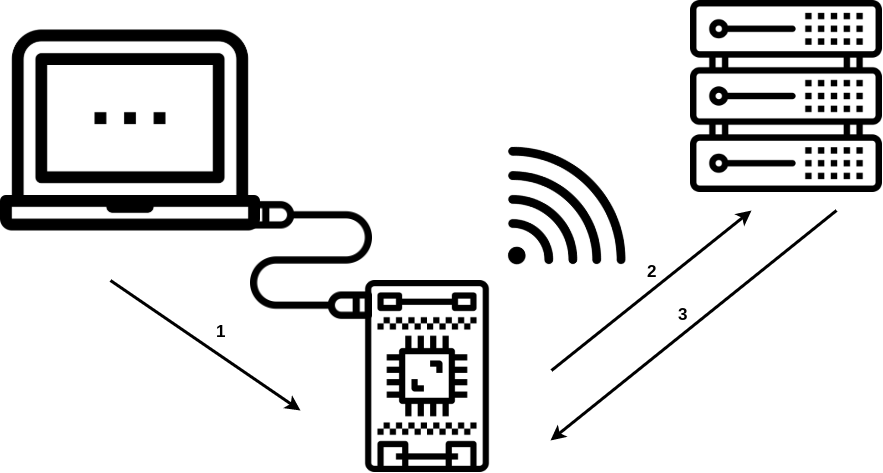
\includegraphics[scale=.5]{images/ota-explanation.png}
        \caption{OTA Erklärung (Quelle: eigene Darstellung)}
    \end{center}    
\end{figure}

\begin{enumerate}
    \item OTA-Enabled Firmware wird zum ersten mal per Kabel auf das Board gespielt
    \item Der Microcontroller schaut nach, ob eine neue Firmware-Version verfügbar ist
    \item Gibt es eine neue Firmware lädt er diese herunter und starte selbst neu
\end{enumerate}

\section{Mesh Netzwerk}\label{sec:mesh}

\section{Nodejs}\label{sec:nodejs}

Nodejs ist eine Laufzeit die auf der Javascript Engine von Chrome aufbaut. Nodejs wurde für das Backend des OTA Servers verwendet.

\subsection{Warum Nodejs?}

Java EE wurde hier nur als ein Beispiel gewählt. Folgendes gilt für jedes Framework das HTTP requests wie JavaEE behandelt. 
Bei der Überlegung welche Sprache bzw. welches Framework für das backend gewählt wird, war die Entscheidung sehr leicht.
Die Anforderungen des OTA Servers sind sehr einfach. Der Server dient nur zur Bereitstellung der Firmwares und beschreibende Informationen über die Firmwares selber.
Da dies nicht CPU intensiv ist sondern I/O intensiv, wurde in diesem Fall Nodejs gewählt.

\subsection{Event Loop}

\subsubsection{Was ist der Event Loop?}

Nodejs selber ist single-threaded deswegen ist der Event Loop einer der wichtigsten Bestandteile von Nodejs.
Der Event Loop erlaubt es nicht-blockenede I/O Operationen durchzuführen. Dies passiert durch die Abladung auf den Kernel von so vielen Operationen wie möglich.
\newline
\newline
Die meisten modernen Kernels sind multi-threaded. Das bedeutet, dass sie mehrere Operationen im Hintergrund unterstützen.

\subsubsection{Wie funktioniert der Event Loop?}

\begin{figure}[H]
    \begin{center}
        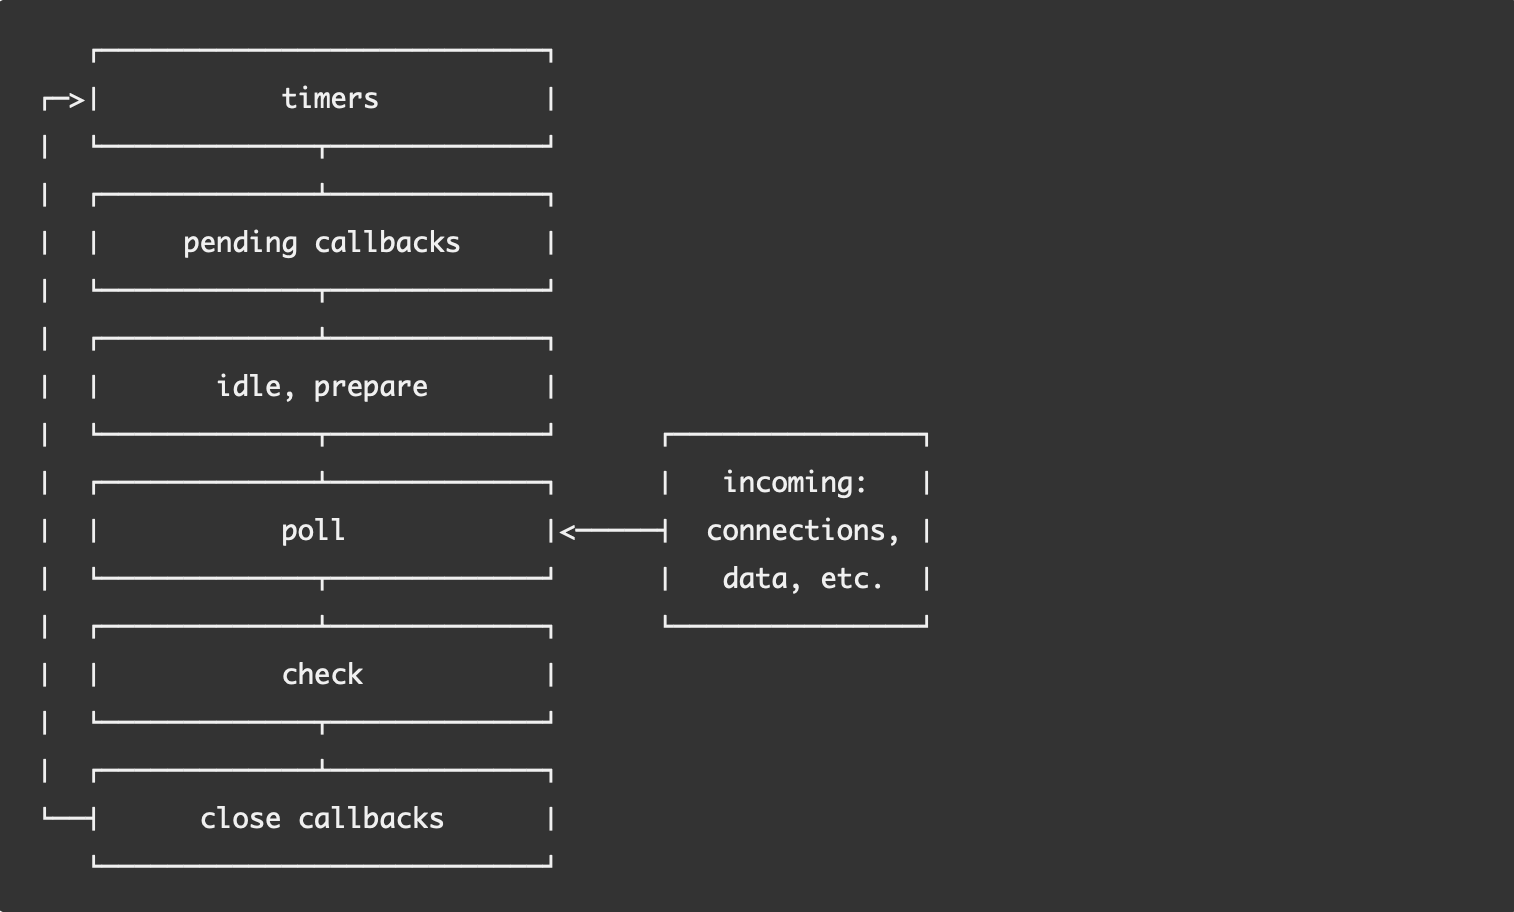
\includegraphics[scale=0.5]{images/nodejs_event_loop.png}
        \caption{Nodejs Event Loop \cite{nodejs_event_loop}}
    \end{center}
\end{figure}

Jeder Block im obigen Bild wird als Phase bezeichnet.
Jede Phase verfügt über eine First-In-First-Out-Warteschlange (FIFO-Warteschlange) mit auszuführenden Rückrufen. 
Während jede Phase auf ihre Weise etwas Besonderes ist, führt sie im Allgemeinen,
wenn die Ereignisschleife in eine bestimmte Phase eintritt, alle für diese Phase spezifischen Operationen aus und führt dann Rückrufe in der Warteschlange dieser Phase aus, 
bis die Warteschlange erschöpft ist oder die maximale Anzahl von Rückrufen ausgeführt hat. 
Wenn die Warteschlange erschöpft ist oder das Rückruflimit erreicht ist, wechselt die Ereignisschleife zur nächsten Phase und so weiter.
\newline
\newline
Da für jeden dieser Vorgänge möglicherweise mehr Vorgänge geplant werden und neue Ereignisse, 
die in der Abfragephase verarbeitet wurden, vom Kernel in die Warteschlange gestellt werden, 
können Abrufereignisse in die Warteschlange gestellt werden, während Abrufereignisse verarbeitet werden. 
Infolgedessen können lange laufende Rückrufe dazu führen, dass die Abfragephase viel länger als der Schwellenwert eines Timers läuft. 

\subsubsection{Phasen}

\begin{itemize}
    \item \textbf{timers:} In dieser Phase werden von setTimeout () und setInterval () geplante Rückrufe ausgeführt.
    \item \textbf{pending callbacks:} führt I/O Callbacks aus, die auf die nächste Iteration verschoben werden
    \item \textbf{idle, prepare:} wird nur intern verwendet
    \item \textbf{poll:} neue I/O Events abrufen; I/O bezogene Callbacks ausführen (fast alle mit Ausnahme von schließ Callbacks, die von Timers geplant werden, und setImmediate ()); Der Knoten wird hier gegebenenfalls blockiert
    \item \textbf{check:} setImmediate() Callbacks werden hier ausgeführt
    \item \textbf{close callbacks:} schließ Callbacks werden ausgeführt
\end{itemize}

Zwischen jedem Durchlauf des Event Loops prüft Nodejs, ob es auf asynchrone I/O oder Timer wartet, und fährt sauber herunter, wenn keine vorhanden sind.

\cite[Zitiert von der offizielen Nodejs Website]{nodejs_event_loop_how_does_it_work}

\section{Platform IO}\label{sec:platformio}

PlatformIO ist ein fortschrittliches und äußerst vielseitiges Ökosystem für die IoT-Entwicklung, das eine IDE, ein Build-System, einen Unified Debugger und einen Bibliotheksmanager umfasst. Es bietet Unterstützung für mehr als 550 Entwicklungsboards, mehr als 25 Entwicklungsplattformen und mehr als 10 nützliche Frameworks. Die PlatformIO IDE ist ein plattformübergreifendes Dienstprogramm für die schnelle berufliche Weiterentwicklung mit integriertem C / C++ - Intelligent Code Completion, Smart Code Linter und erweitertem Serial Port Monitor. PlatformIO kann auch in die gängigen IDEs und kontinuierlichen Integrationssysteme integriert werden, um die Zeit für die Bereitstellung von IoT-Anwendungen zu verkürzen.\cite{platformio_about_us}

PlatformIO ist in reinem Python geschrieben und hängt nicht von zusätzlichen Bibliotheken / Tools eines Betriebssystems ab. So kann man mit PlatformIO auf Windows, Macintosh und Linux arbeiten.

\section{ESP IDF Toolchain}\label{sec:platformio}

\section{Docker}\label{sec:docker}

\section{Docker Compose}\label{sec:docker-compose}

Docker-compose ist ein Tool zum Definieren und Ausführen von Docker-Anwendungen mit mehreren Containern. Mit Compose verwenden Sie eine YAML-Datei, um die Dienste Ihrer Anwendung zu konfigurieren. Anschließend erstellen und starten Sie mit einem einzigen Befehl alle Dienste in Ihrer Konfiguration. \cite{docker_compose_description}

\subsection{Docker Compose Beispiel}

\begin{figure}[H]
    \begin{center}
        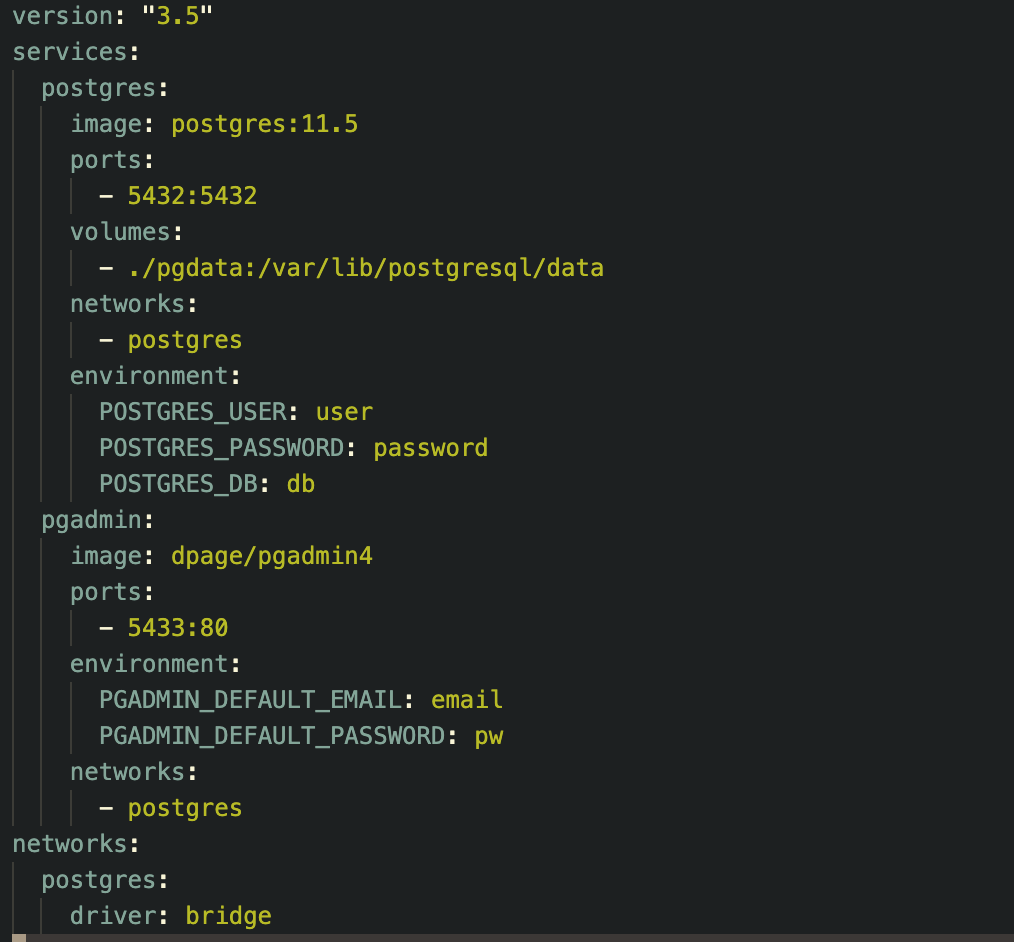
\includegraphics[scale=0.8]{images/docker_compose_example.png}
        \caption{Docker Compose Beispiel}
    \end{center}
\end{figure}

In der obigen Abbildung kann man das docker-compose.yml file von dem OTA Server sehen.

Die Struktur eines docker-compose files ist im Normalfall immer gleich. Am Anfang definiert man welche Version des Standards man verwendet und anschließend die verschiedenen Dienste. Der OTA Server benötigt nur 2 Dienste:

\begin{enumerate}
    \item Postgres
    \item PgAdmin4
\end{enumerate}

% Da beide Dienste miteinander kommunizieren müssen, sind beide in dem selben Netzwerk namens \textit{postgres}.

In diesem Beispiel wird das Netzwerk explizit erstellt. Es ist auch möglich das Netwerk implizit zu erstellen, indem man den networks Bereich von ganz unten entfernt.

\subsubsection{Postgres}

Datenbank für die Speicherung von den Informationen über die verschieden Firmwares die gerade auf dem Server hochgeladen sind.

Die Datenbank braucht irgendeinen Weg um mit der Außenwelt kommunizieren zu können, deswegen wird der interne Port 5432 auf den externen Port 5432 geleitet.

Damit die Absicherung der Datenbank leicht verläuft wird ein Volume für die Datenbank erstellt, worin sich die Daten der Datenbank befinden. In dieser docker-compose Datei wird das Volume implizit erstellt. 

Man kann es auch explizit erstellen wie folgt:

\begin{verbatim}
    volumes:
        pgdata:
\end{verbatim}

Mit den Umgebungsvariablen kann man die Standardwerte überschreiben. Die Datenbank hat in der obigen Abbildung den Benutzer \textit{user} mit dem Passwort \textit{password} und der default Datenbank \textit{db}.

\subsubsection{PgAdmin4}

PgAdmin4 ist eine web-basierte Benutzeroberfläche für Postgres.

Sie ist die PhpMyAdmin Oberfläche in der postgres Welt.

Die Software binded automatisch auf den Port 80, was für Entwicklungszwecke sehr unpraktisch ist, da Port 80 auf Ubuntu zum Beispiel Adminrechte benötigt. Deswegen wird der interne Port 80 auf den externen Port 5433 umgeleitet.

Mit den Umgebungsvariablen \textit{PGADMIN\_DEFAULT\_EMAIL} und 
\textit{PGADMIN\_DEFAULT\_PASSWORD} werden die default Logindaten für PgAdmin4 definiert. 

\section{ESP IDF Utility lib}\label{sec:esp-idf-utility-lib}

\section{React}\label{sec:react}

\section{Yarn}\label{sec:yarn}

\section{Webpack}\label{sec:webpack}
